\documentclass[%draftcls, journal
]{IEEEtran}

\usepackage{graphicx}
\usepackage{hyperref}
\usepackage[caption=false,font=footnotesize]{subfig}
\usepackage{listings}

%set listings defaults
\lstset{
 basicstyle=\small,
 showstringspaces=false,
 language=c++
}

\begin{document}

\title{Homework 8 Report}
\author{Jane~Doe% 
\thanks{Undergraduate Student, Department of Astronautical Engineering}%
}
\markboth{Homework 8}{}%
\maketitle

\begin{abstract}
This report summarizes work performed for HW 8 in Class XYZ.
\end{abstract}

%-------------------
\section{Introduction}
Here is a quick summary of what was done on this homework assignment. We started by writing code to perform some matrix operation on vectors $\vec{a}$ and $\vec{b}$. We defined the \emph{dot} operation

\begin{equation}
\vec{a}\cdot\vec{b} = \sum_{i=0}^2 a_i b_i = a_0b_0 + a_1b_1 + a_2b_2
\end{equation}

We also defined the \emph{mag} operation,
\begin{equation}
\left|\vec{a}\right| = \sqrt{\vec{a}\cdot\vec{a}}
\label{e:mag}
\end{equation}
The equation shown in \ref{e:mag} is coded up as

\begin{lstlisting}
friend double mag(const _vec3<T>&a) {
  return sqrt(dot(a,a));
}
\end{lstlisting}

\section{Source Control}
We setup a Github repo, as shown in Figure \ref{f:repo}.

\begin{figure}[h]
\centering
{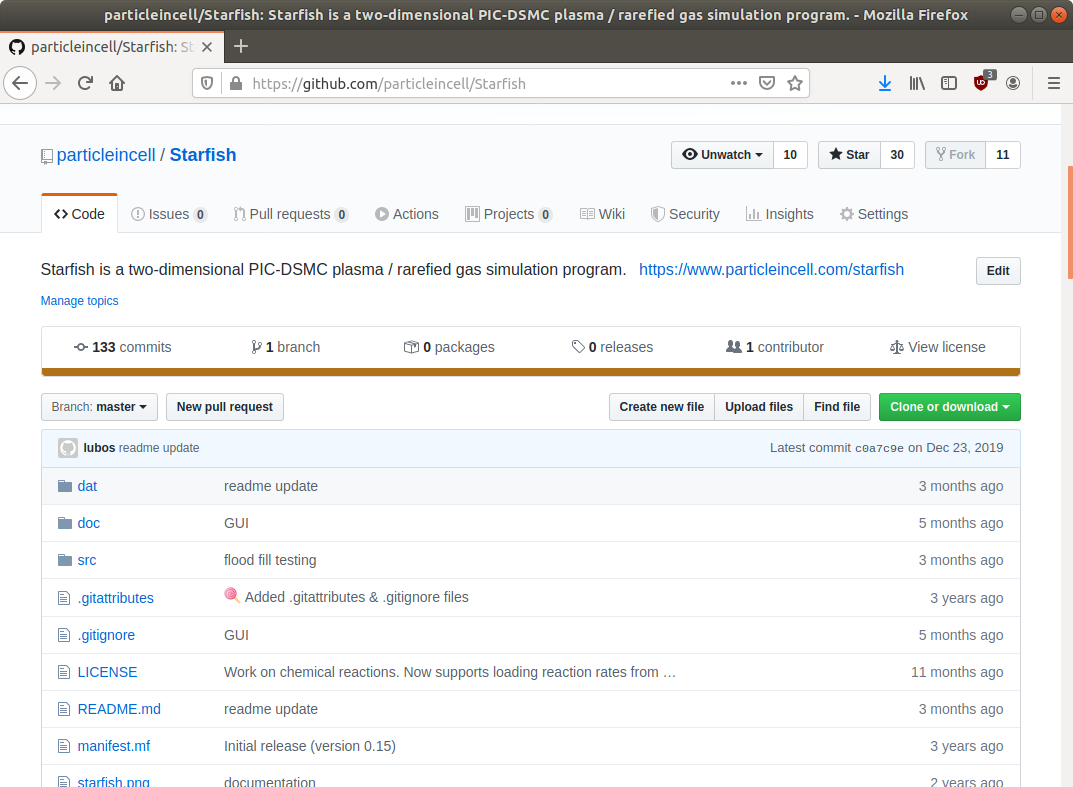
\includegraphics[width=0.8\linewidth]{github}}  %this requires github.png
\caption{Screenshot of the brand new Github repo}
\label{f:repo}
\end{figure}

We also learned how to use \href{http://doxygen.nl/manual/docblocks.html}{Doxygen}, \texttt{Google Test}, and \LaTeX.  These tools are summarized in Table \ref{t:techs}.
Article by A. Somebody provides a good overview \cite{somebody} of these tools.

\begin{table}[t]
\centering
\caption{Summary of technologies}
\label{t:techs}
\begin{tabular}{l|l}
\textbf{Technology} & \textbf{Use}\\ %add new line
\hline
Doxygen & Developer guide documentation system \\
GTest & Unit Testing for C++ \\
Github & Source Control Repository \\
LaTeX & Technical paper writing language
\end{tabular}
\end{table}

\section{Conclusion}
There was no programming in this homework so it was very easy!

\section*{Acknowledgment}
I took advantage of the professor's office hour for help on this assignment.

\bibliographystyle{ieeetr}
\bibliography{ex8}
\end{document}
